% Adjust these for the path of the theme and its graphics, relative to this file
%\usepackage{beamerthemeFalmouthGamesAcademy}
\usepackage{../../beamerthemeFalmouthGamesAcademy}
\usepackage{multimedia}
\graphicspath{ {../../} }

% Default language for code listings
\lstset{language=C++,
        morekeywords={each,in,nullptr}
}

% For strikethrough effect
\usepackage[normalem]{ulem}
\usepackage{wasysym}
\usepackage{graphicx} %package to manage images

\usepackage{pdfpages}

% http://www.texample.net/tikz/examples/state-machine/
\usetikzlibrary{arrows,automata}


\newcommand{\modulecode}{COMP702}\newcommand{\moduletitle}{Classical Artificial Intelligence}\newcommand{\sessionnumber}{1}

\begin{document}
\title{\sessionnumber: Ideation Techniques}
\subtitle{\modulecode: \moduletitle}

\begin{frame}
	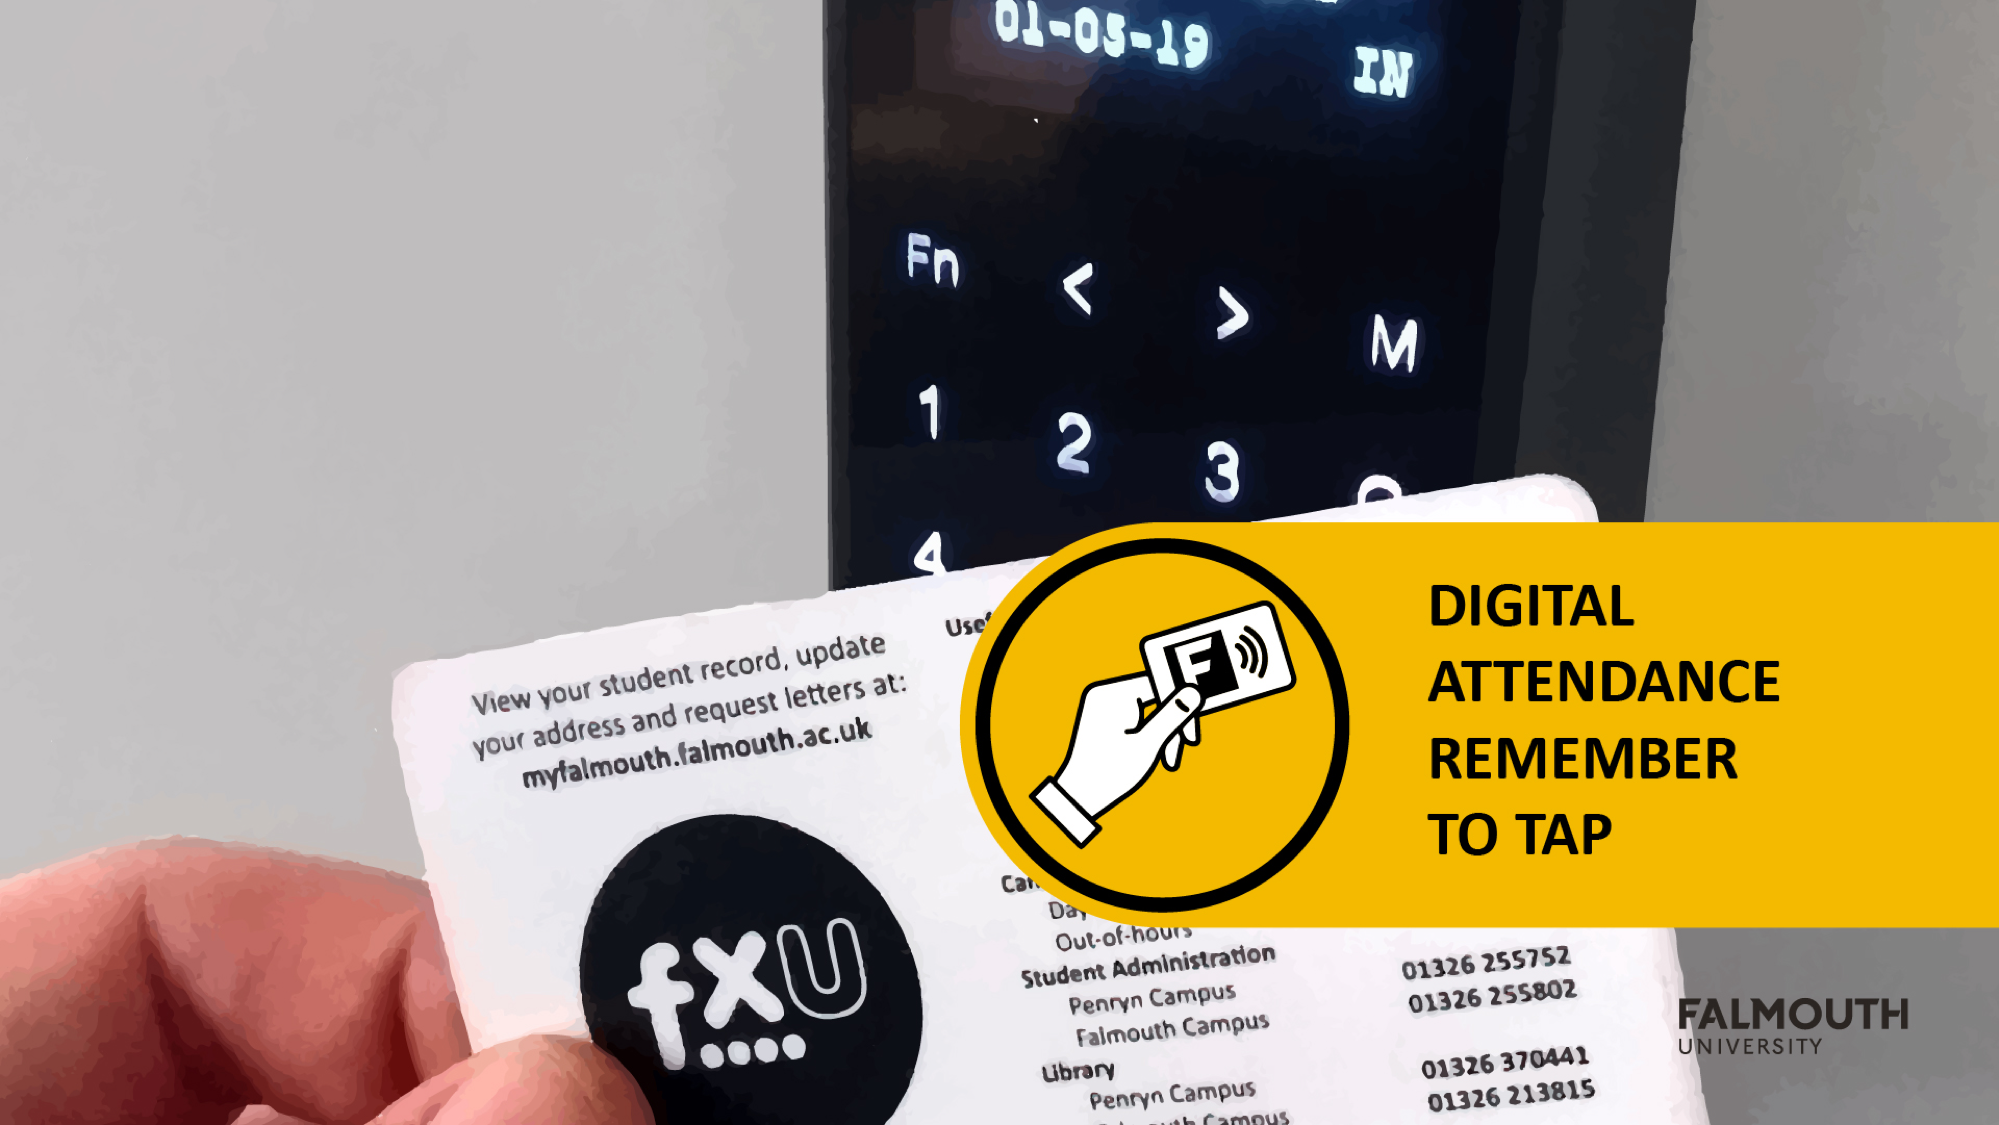
\includegraphics[width=1.0\textwidth]{sign-in}
\end{frame}

\frame{\titlepage} 


\begin{frame}{Today's agenda}
	\begin{itemize}
		\item Ideation techniques
		\item and how we can use them to come up with ideas
	\end{itemize}
\end{frame}

\end{document}
